\documentclass[rebuttal]{cvpr}

\usepackage{times}
\usepackage{epsfig}
\usepackage{graphicx}
\usepackage{amsmath}
\usepackage{amssymb}

% Include other packages here, before hyperref.

% If you comment hyperref and then uncomment it, you should delete
% egpaper.aux before re-running latex.  (Or just hit 'q' on the first latex
% run, let it finish, and you should be clear).
\usepackage[pagebackref=true,breaklinks=true,colorlinks,bookmarks=false]{hyperref}

%%%%%%%%% PAPER ID  - PLEASE UPDATE
% \def\cvprPaperID{****} % *** Enter the CVPR Paper ID here
%\def\httilde{\mbox{\tt\raisebox{-.5ex}{\symbol{126}}}}

\def\cvprPaperID{****} % *** Enter the CVPR Paper ID here
\def\confYear{CVPR 2024}

\begin{document}

%%%%%%%%% TITLE - PLEASE UPDATE
\title{Real and Fake Face Detection}  % **** Enter the paper title here

\maketitle
\thispagestyle{empty}


%%%%%%%%% BODY TEXT - ENTER YOUR RESPONSE BELOW
\section{Abstract}
In this project, our primary aim is to compile a comprehensive dataset consisting of genuine and altered human facial images. Subsequently, we seek to develop a convolutional neural network (CNN) capable of discerning fabricated images within this dataset. Our focus extends to evaluating the performance of our CNN model against established benchmarks, including the simple and improved CNN model, pre-trained MobileNetV2, and GramNet (with Gram Block). Through meticulous data collection and model development processes, we aim to provide insights into the efficacy of various CNN architectures for detecting manipulated images. Throughout model development, we experiment with various CNN architectures, exploring differences in depth, layer types, and regularization methods. We benchmark our CNN model against different models using different datasets.
 

\section{Introduction}

In the era of advanced digital manipulation technologies, the proliferation of fake images, particularly of human faces, has become a prevalent concern, demanding robust detection methods capable of discerning between genuine and altered facial images. Our project responds to this challenge by compiling a comprehensive dataset comprising both authentic and manipulated human facial images, leveraging which we aim to develop a convolutional neural network (CNN) capable of accurately identifying fabricated images. With our primary focus on the development of a CNN tailored for fake face detection, we explore various architectures including ResNet, MobileNetV2, and GramNet with Gram Block, to discern their efficacy in detecting manipulated images. Through systematic experimentation, we delve into architectural differences such as depth, layer types, and regularization methods, with the goal of optimizing model performance.
 
Dataset Compilation:
To construct our dataset, we draw upon the "Real and Fake Face Detection" dataset sourced from Kaggle. This dataset offers a diverse collection of genuine and altered facial images, providing a suitable foundation for training and evaluation purposes. By meticulously curating and augmenting this dataset, we ensure a broad representation of facial variations and manipulation techniques, facilitating robust model training.
 
Benchmarking Against Established Models:
To assess the effectiveness of our CNN model, we benchmark its performance against established baselines, including ResNet and MobileNetV2, renowned for their accuracy and efficiency in image classification tasks. Furthermore, we compare our model against GramNet with Gram Block, a state-of-the-art approach noted for its robustness and general applicability in fake face detection. By conducting rigorous evaluations using identical test datasets, we provide insights into the relative strengths and weaknesses of different CNN architectures for detecting manipulated images.

%-------------------------------------------------------------------------

\subsection{Sample}
Sample

%------------------------------------------------------------------------
\section{Related Work}
\section{Method}

\subsection{Convolutional Neural Network}

A simple CNN network can be used to test the correctness of program exectution and observe the flow of data. Because of its brief structure, it can significantly reduce the cost of computing resources. At the same time, it can alos be used as one of the benchmark performance indicators for comparison and analysis with other types of subsequent network models.

This convolutional neural network is designed for image classificaion, structured with an input layer which taks 3-channel RGB images, followed by three convolutional layers, each with a 3x3 kernal and padding of 1, progressively increasing the number of filters from 32 to 64 and finally 128. Each convolutional layer is followed by a ReLU activation function and a 2x2 max pooling layer. The output is flattened and passed throught two fully connected layers. The first FC layer transforms the feature map into 512 features, followed by another ReLU, and the second FC layer reduces it to 2 outputs for classification. 

The Improved CNN represents an enhancement of the previous 'SimpleCNN' model. it is designed to achieve better performance by adopting serveral architectural adjustments to increase the network's capacity and reduce overfitting.

Compared with the basic version of CNN, the improved version of convolutional neural network has been improved in the following aspects: An additional convolutional layer has been introduced; The depth is increased with 256 filters; Each convolutional layer is now followed by a batch normalization layer; A dropout layer with a rate is introduced before the first fully connected layer; Also an increased fully connected layer capacity, transforms the feature maps into a larger dimensional space.

\subsection{GramNet Architecture}
In the GramNet architecture (Figure 2), Gram Blocks (Figure 1) are integrated at the input image stage and before each downsampling layer to encapsulate global image texture information across various semantic levels. Each Gram Block is composed of several layers: an initial convolution layer adjusts the feature dimensions from diverse levels, followed by a Gram matrix calculation layer that captures the global image texture features. This setup is then refined through two consecutive layers—each a combination of a convolution, a batch normalization, and a ReLU activation. Finally, a global pooling layer is employed to synchronize the gram-style features with the main ResNet like framework.

\begin{figure}[t]
\begin{center}
   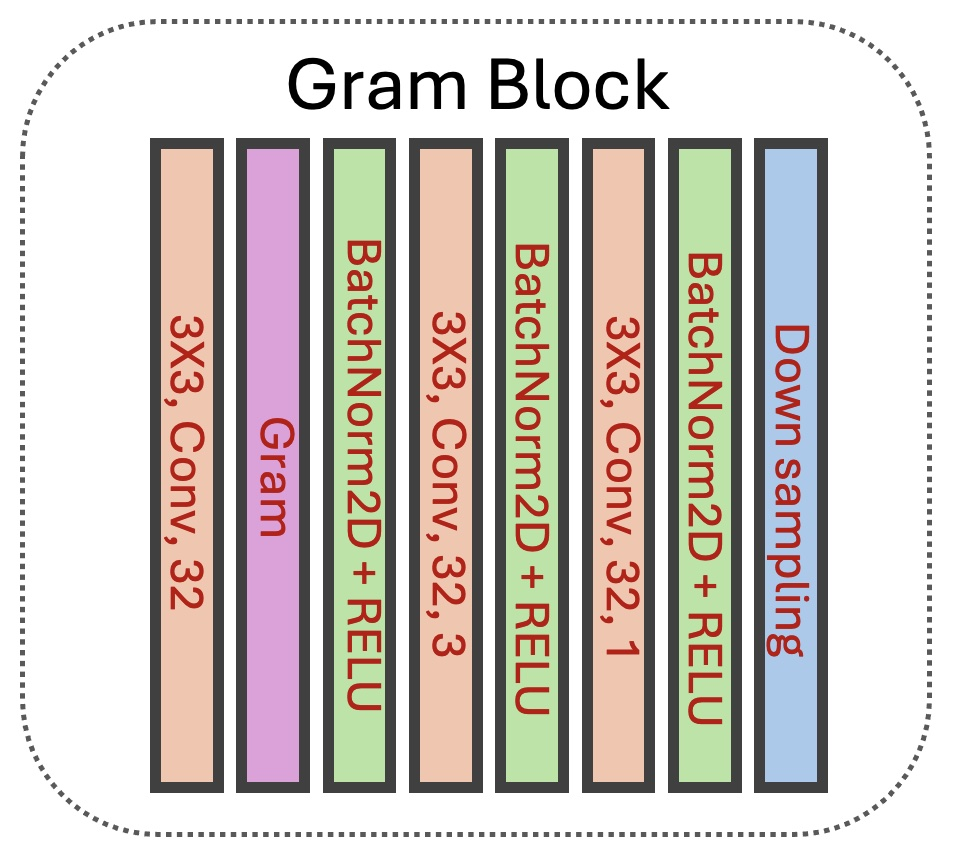
\includegraphics[width=0.8\linewidth]{GramBlock.jpg}
\end{center}
   \caption{Gram Blocks are added to the GramNet architecture on the input image and before every downsampling layer, incorporating global image texture information in different semantic levels. In the Gram Block, there are three convolutional layers, and for each convolutional layer, we apply Batch Normalization and Relu active function to it. In the end, we use the downsampling layer.}
\label{fig:long}
\label{fig:onecol}
\end{figure}

\begin{figure*}[t]
\begin{center}
   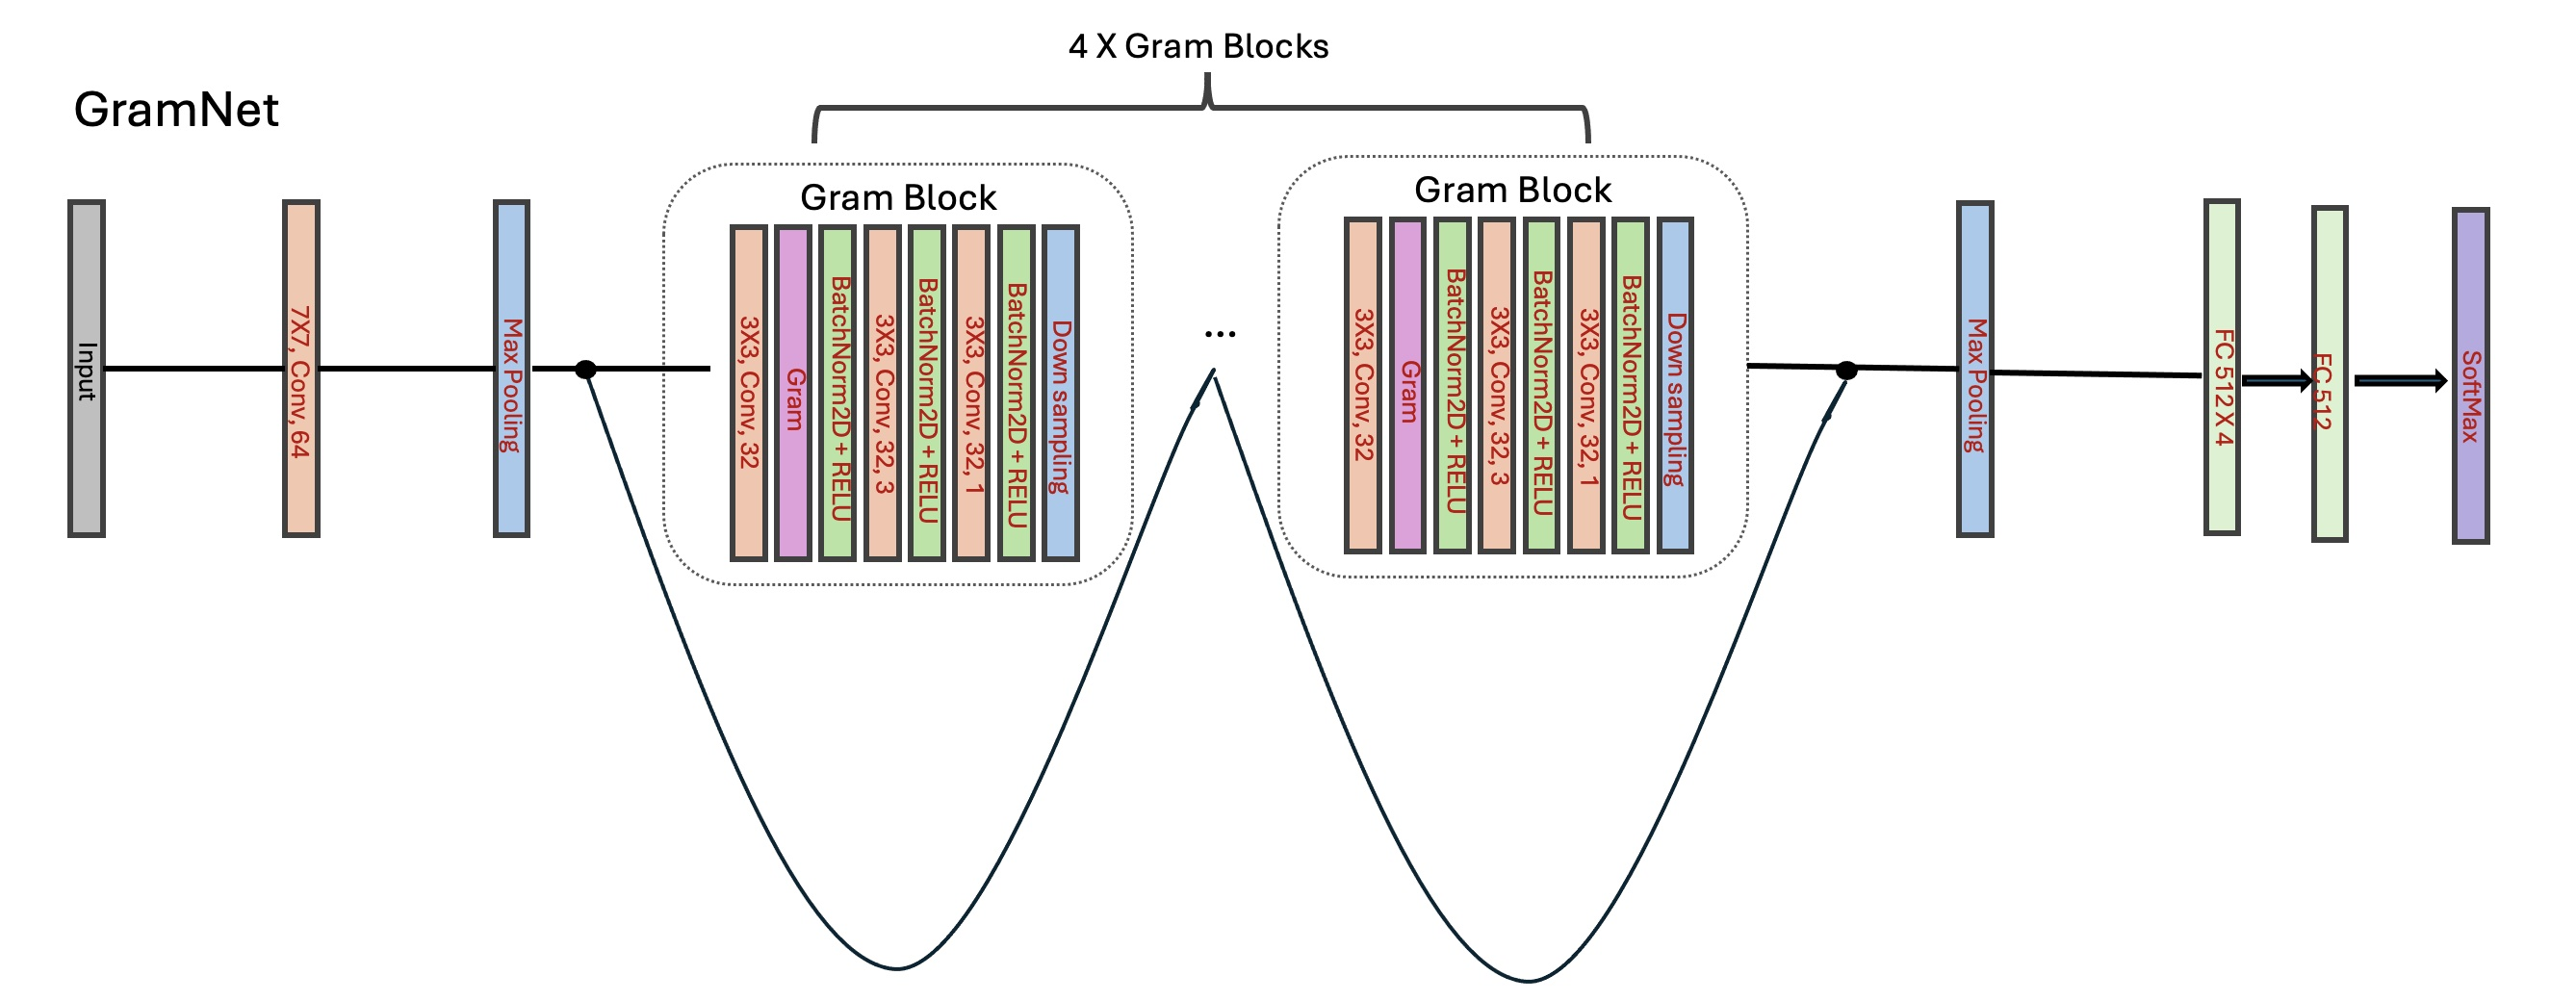
\includegraphics[width=0.8\linewidth]{GramNet.jpg}
\end{center}
   \caption{In the GramNet architecture, Gram Blocks are strategically integrated to enhance the capture of global features.}
\label{fig:long}
\label{fig:onecol}
\end{figure*}

In designing this model, there are three primary reasons for its architectural choices:  

\textbf{Enhanced Capture of Global Texture Features:} Unlike traditional models that predominantly focus on local features extracted from feature maps, this model is designed to capture more global texture features. By integrating Gram Blocks within the ResNet architecture, the model effectively incorporates global information at various semantic levels. This approach is particularly beneficial for tasks like distinguishing real from fake faces, where understanding the overall texture and coherence of the image is crucial.
\\
\\
\textbf{Increased Accuracy and Robustness:} The addition of Gram Blocks aims to enhance the model's accuracy and robustness. By enriching the feature set with both local and global descriptors, the model gains a more comprehensive understanding of the image content, which leads to improved performance on complex image recognition tasks.
\\
\\
\textbf{Increased Computational Demand:} The introduction of Gram Blocks, especially the computation of the Gram matrix and subsequent layers, adds substantial computational overhead. This increase in complexity means that more time and resources are required for training the model, which could be a limiting factor depending on the available computational power and the efficiency requirements of the application.

\section{Experiments}
\subsection{Datasets}
\begin{itemize}
    \item Dataset 1: Real-and-fake-detection image dataset  \\
    Source: https://www.kaggle.com/datasets/ciplab/real-and-fake-face-detection?resource=download \\
    For this dataset used in real and fake image detection, the training set comprises 1,081 real images and 960 fake images.
    \item Dataset 2: Deepfake-and-real image dataset  \\
    Source: https://www.kaggle.com/datasets/manjilkarki/deepfake-and-real-images/discussion \\
    This dataset, designed for the evaluation of real and fake image detection algorithms, is comprehensive and well-structured. It encompasses distinct subsets for training, validation, and testing, featuring both real and fake images. Each image within the dataset is a 256x256 pixel JPEG depicting a human face, categorized as either authentic or counterfeit. Overall, the dataset comprises a substantial total of 190,000 human face images.

    \item Glimpse of our dataset: As it shows in Figure 3, we could the sample fake and real faces from our dataset 1.
    
\begin{figure*}[t]
\centering
\begin{minipage}{0.45\linewidth}
   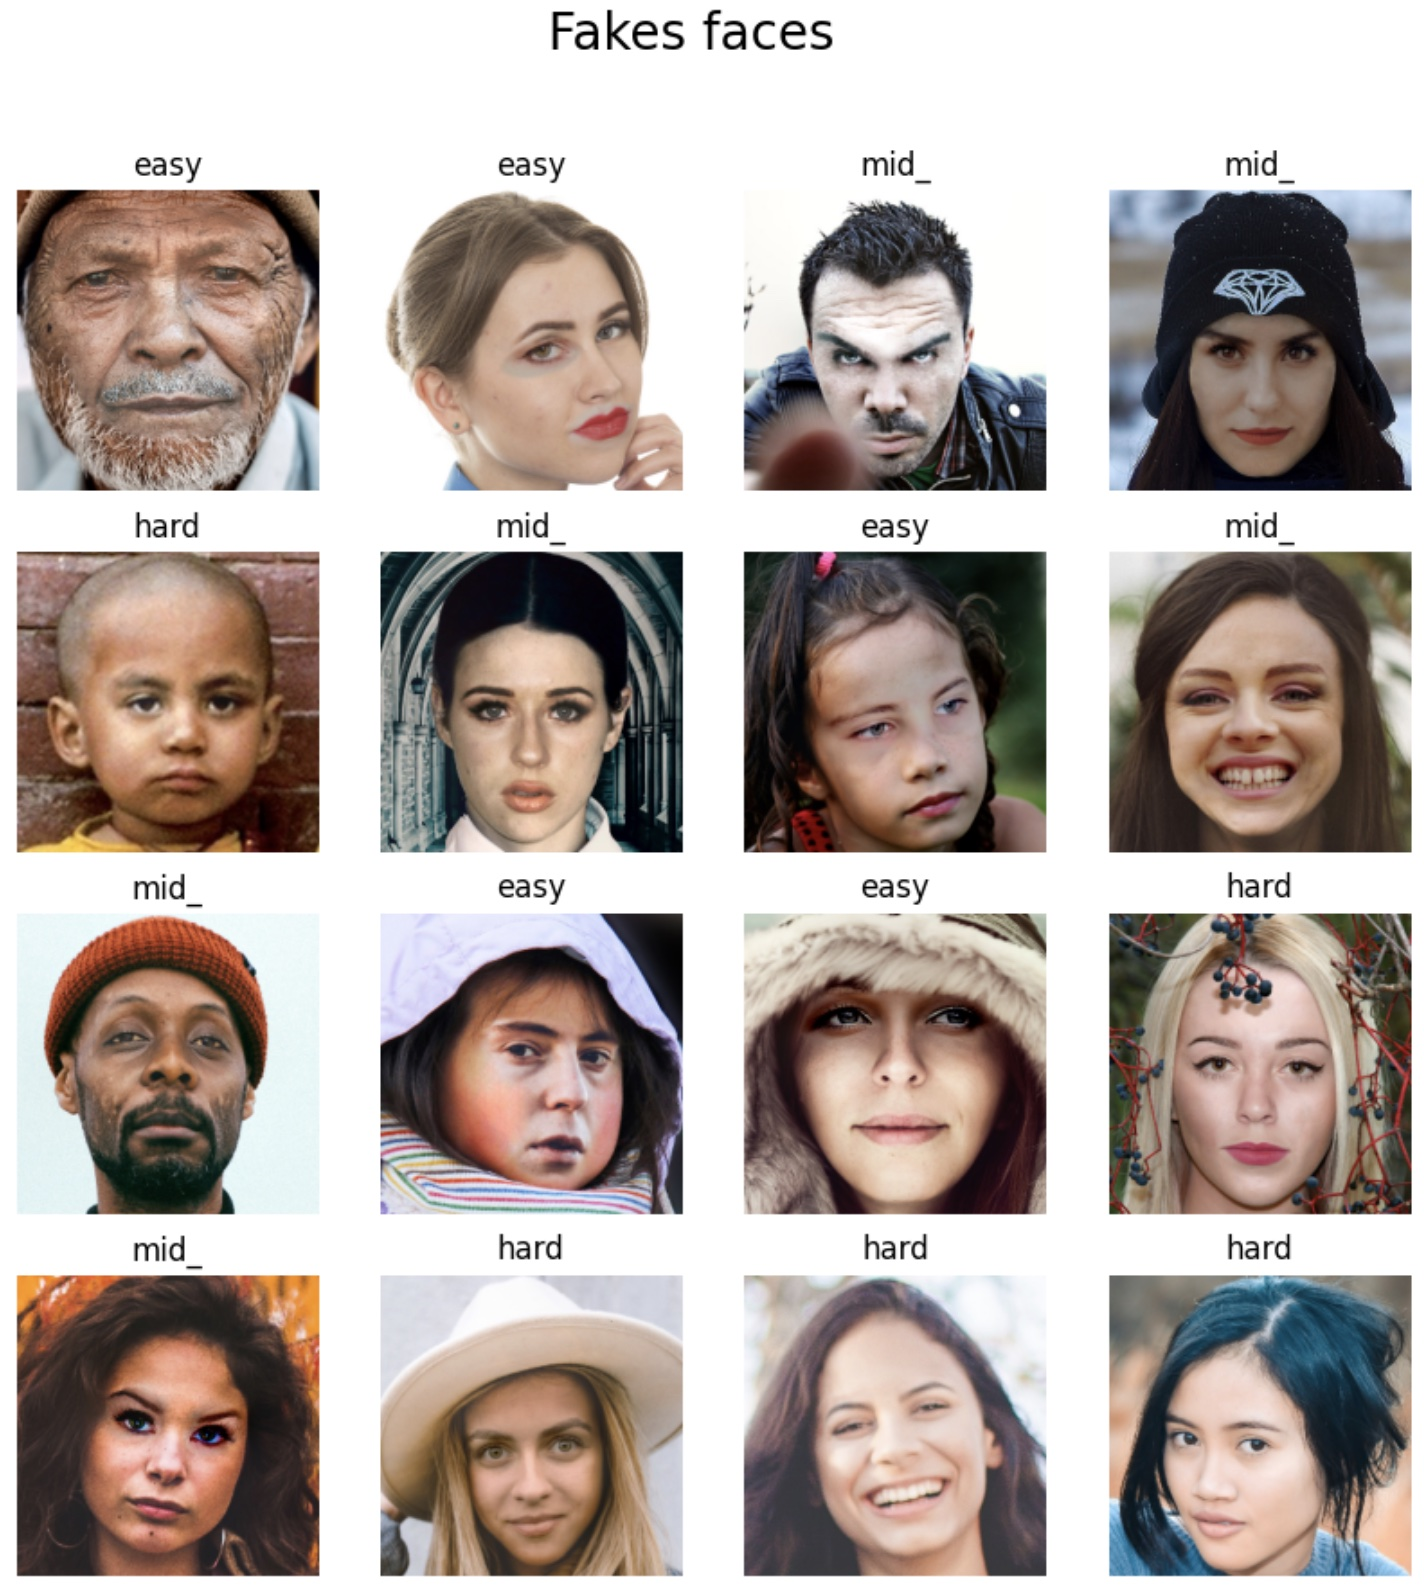
\includegraphics[width=\linewidth]{Dataset1_Fakeface.jpg}
   % \caption{Fake faces from dataset 1}
   \label{fig:image1}
\end{minipage}
\hfill
\begin{minipage}{0.45\linewidth}
   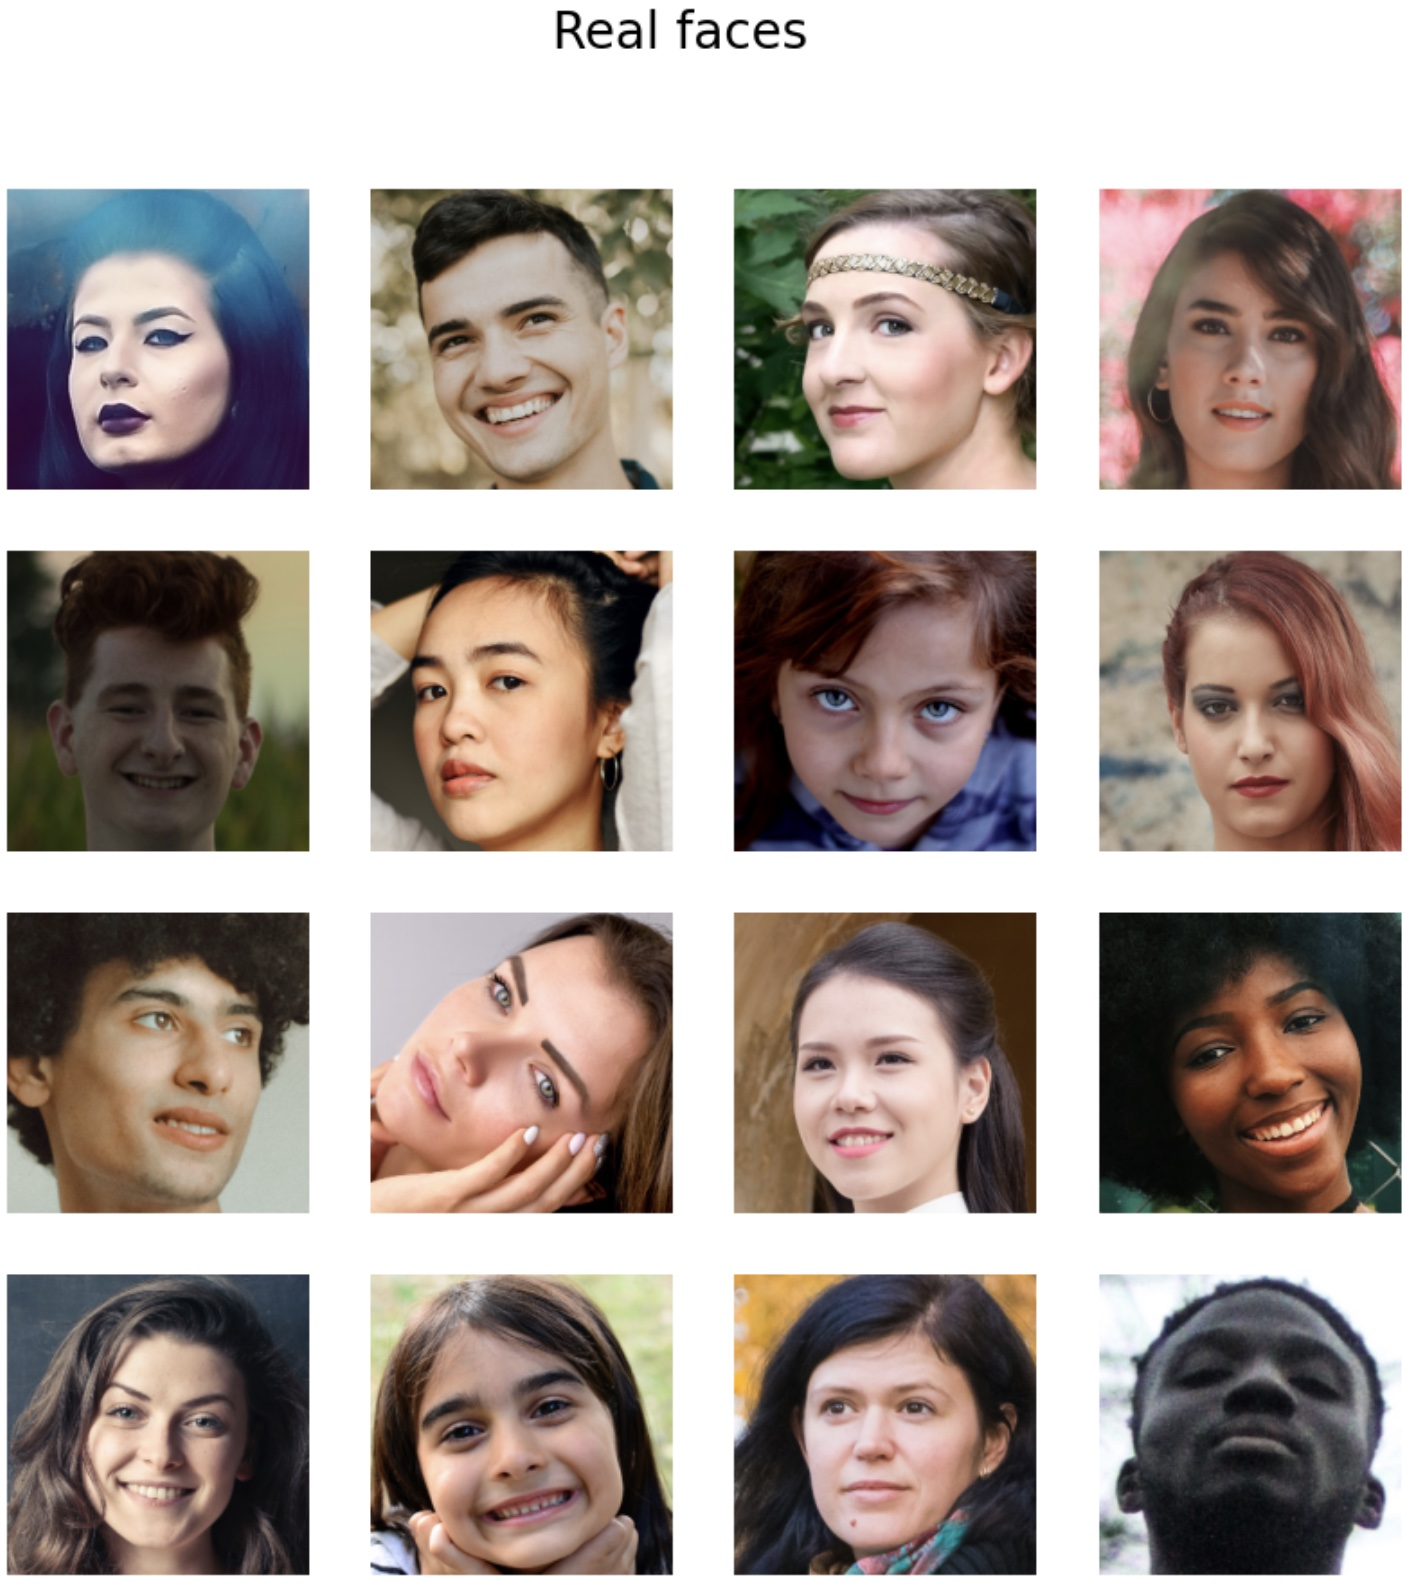
\includegraphics[width=\linewidth]{Dataset1_Realface.jpg}
   % \caption{Real faces from dataset 1}
   \label{fig:image2}
\end{minipage}
\caption{Glimpse of the dataset}
\label{fig:dataset}
\end{figure*}
\end{itemize}


\subsection{Details in Experiment}
\subsubsection{Model training and evaluation}
\begin{itemize}
        \item Simple CNN \\
         1. Training and validating on dataset 1
            Experienments start with the small-scale dataset 1, wiit simpleCNN structure, as in Figure~\ref*{fig:ex-d1-simplecnn-results}, after 20 rounds of iterations, the validation accuracy remains fluctuating within a range and has not increased significantly. The accuracy is about 60\%.
            \\
            \\
         2.Training and validating on dataset 2
            The situation changes when large-scale data sets are adopted. With the support of the training set of 140k+ images, even the network structure of simpleCNN has achieved a huge leap in verification accuracy. As shown in Figure~\ref*{fig:ex-d2-simplecnn-results}, it reached about 94\% after 20 rounds of iterations. Compared with the case of using the simplified data set (Figure~\ref*{fig:ex-d1-simplecnn-results}), an improvement of more than 30\% is achieved.
        
        \begin{figure}[t]
           \centering
           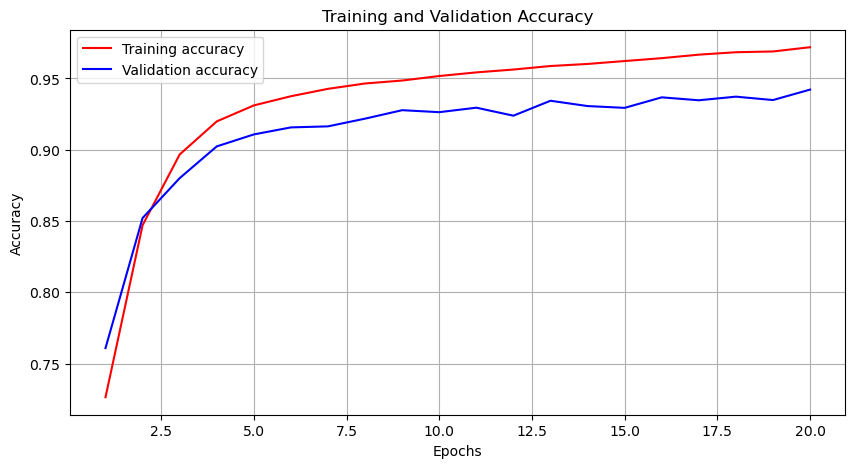
\includegraphics[width=0.9\linewidth]{images/ex-d2-simplecnn-accuracy-results.png}
           \caption{Training and Validation results of simple CNN with the large-scale dataset}
           \label{fig:ex-d2-simplecnn-results}
        \end{figure}
        
        \begin{figure}[t]
           \centering
           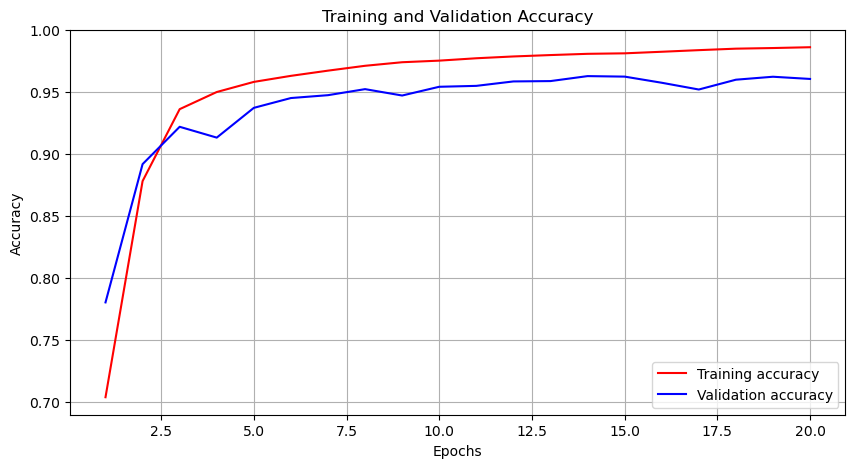
\includegraphics[width=0.9\linewidth]{images/ex-d2-improvedcnn-accuracy-results.png}
           \caption{Training and Validation results of improved CNN with the large-scale dataset}
           \label{fig:ex-d2-improvedcnn-results}
        \end{figure}
        \begin{figure}[t]
           \centering
           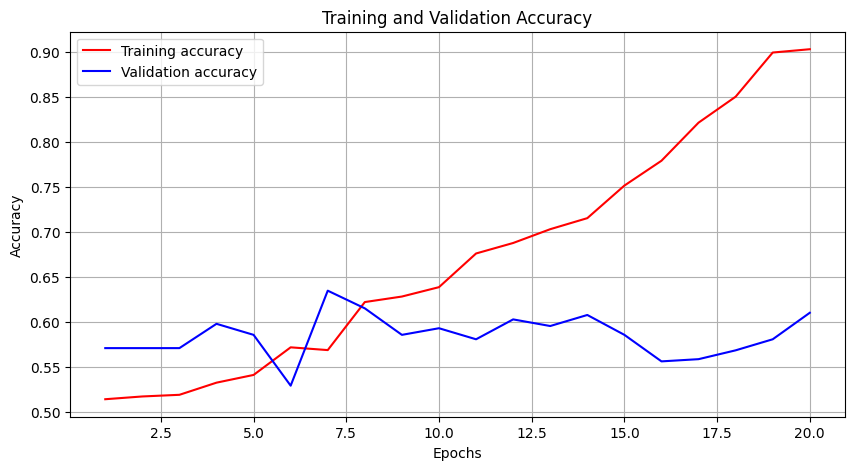
\includegraphics[width=0.9\linewidth]{images/ex-d1-simplecnn-accuracy-results.png}
           \caption{Training and Validation results of simple CNN with the compact dataset}
           \label{fig:ex-d1-simplecnn-results}
        \end{figure}
        
        \begin{figure}[t]
           \centering
           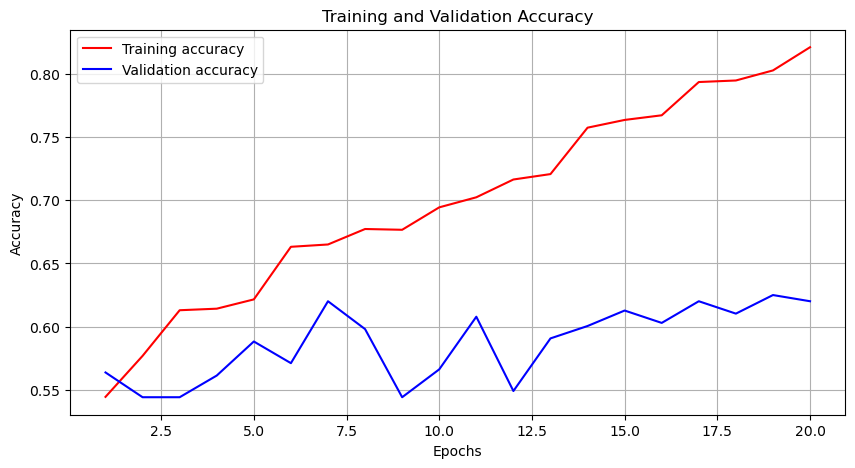
\includegraphics[width=0.9\linewidth]{images/ex-d1-improvedcnn-accuracy-results.png}
           \caption{Training and Validation results of improved CNN with the compact dataset}
           \label{fig:ex-d1-improvedcnn-results}
        \end{figure}
        
        \item Improved CNN \\
        1. Training and validating on dataset 1
            The ImprovedCNN brought slight better performance in the later iterations of training. As shown in Figure~\ref*{fig:ex-d1-improvedcnn-results}, the validation accuracy range came to between 60\% to 65\%, but it was very unobvious and thus did not bring significantly improvement.
            \\
            \\
        2.Training and validating on dataset 2 
            The performance of the improved CNN network structure in large-scale datasets is shown in Figure~\ref*{fig:ex-d2-improvedcnn-results}. Although it has been greatly improved, the advantage over simpleCNN is very little. after 20 epochs, it reached about 96\% validation accuracy.

        \item GramNet \\
        1. Training and validating on dataset 1
            In the case of Dataset 1, as shown in Figure 4, which is characterized by its limited size, the GramNet architecture fails to demonstrate its effectiveness. The constrained volume of training data appears to significantly hinder the model's performance, resulting in notably poor outcomes on this dataset. This observation underscores the potential limitations of GramNet when applied to smaller datasets, where insufficient training examples may not adequately support the complex feature extraction capabilities designed to harness global image texture information.   
            \\
            \\
        2. Training and validating on dataset 2
           Conversely, when applied to Dataset 2, as shown in Figure 5, the GramNet architecture exhibits markedly improved performance compared to Dataset 1. This enhancement is primarily attributed to the larger volume of data incorporated into the model for training. The increased dataset size provides a more robust foundation for the GramNet to effectively leverage its sophisticated mechanisms for global feature extraction, thus resulting in superior outcomes. This contrast highlights the importance of adequate training data in realizing the full potential of advanced neural network architectures like GramNet.
            \\
            \\
        3. Training and validating on cross-dataset
            Subsequently, we implemented cross-dataset training and validation to enhance the generalization capabilities and robustness of our model, as shown in Figure 6. This approach involved training the model on one dataset and validating it on another, aiming to ascertain its performance across different data distributions. The results were highly encouraging, as the model achieved significant accuracy and minimal loss, surpassing the performance observed when trained solely on a single dataset. These findings underscore the efficacy of cross-dataset training in bolstering the adaptability and overall performance of the model.
        \item MobileNetV2 \\
         Regarding the application of the pre-trained MobileNetV2, the model was trained and validated across both Dataset 1 and Dataset 2, as well as in cross-dataset scenarios. It became evident that MobileNetV2 possesses robust generalization capabilities, particularly in the detection of facial features. In cross-dataset evaluations, MobileNetV2 achieved an accuracy rate of 0.98, which marginally surpasses that of GramNet51. Additionally, it is noteworthy that MobileNetV2 has fewer trainable parameters, which contributes to its efficiency and effectiveness in generalization compared to more complex models.
\end{itemize}

% Training and validating for various models
\begin{figure*}[t]
\centering
\begin{minipage}{0.45\linewidth}
   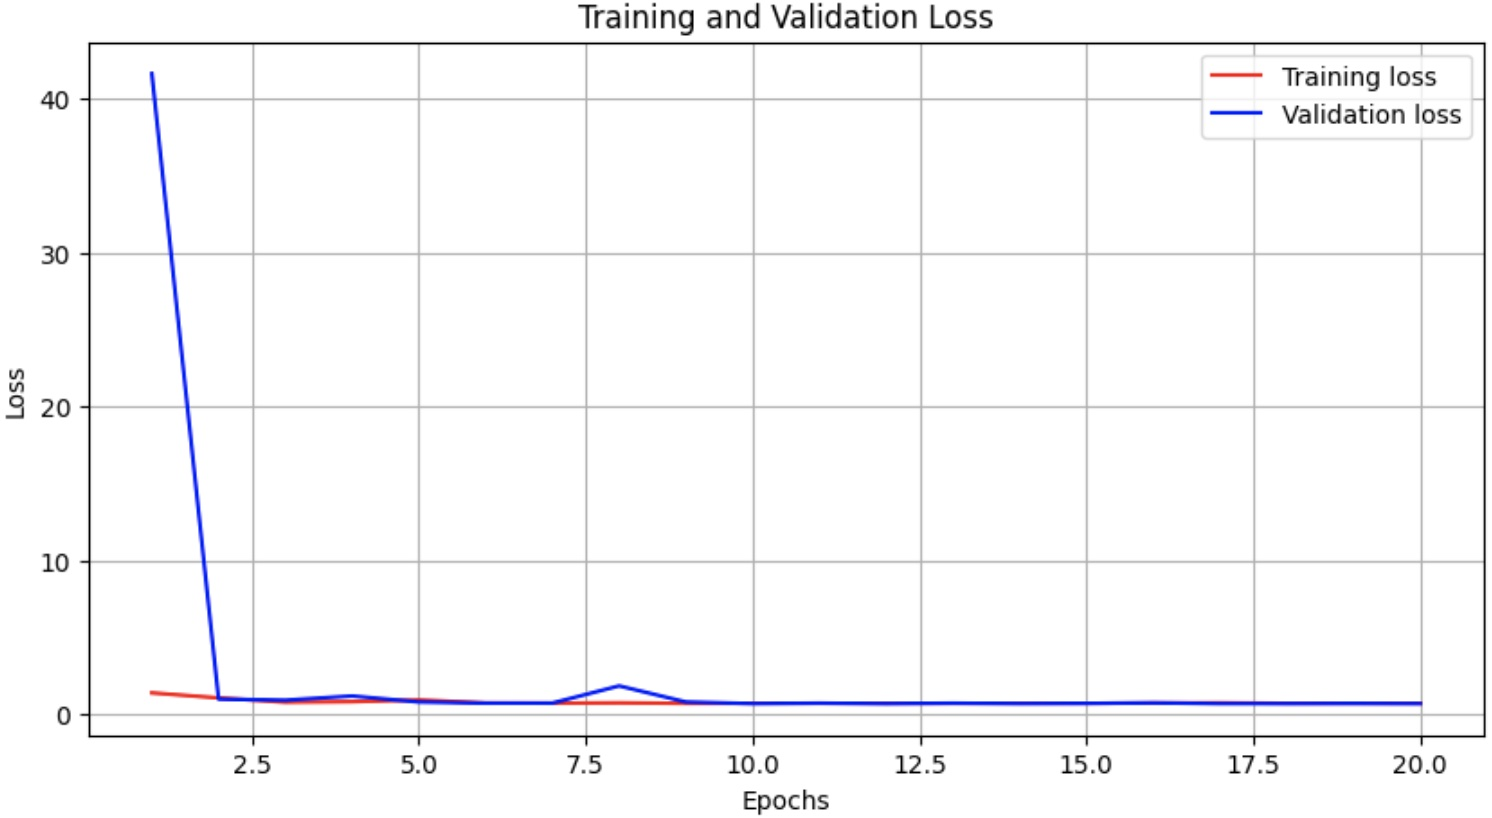
\includegraphics[width=\linewidth]{gramnet51_d1_loss.jpg}
   % \caption{Fake faces from dataset 1}
   \label{fig:image1}
\end{minipage}
\hfill
\begin{minipage}{0.45\linewidth}
   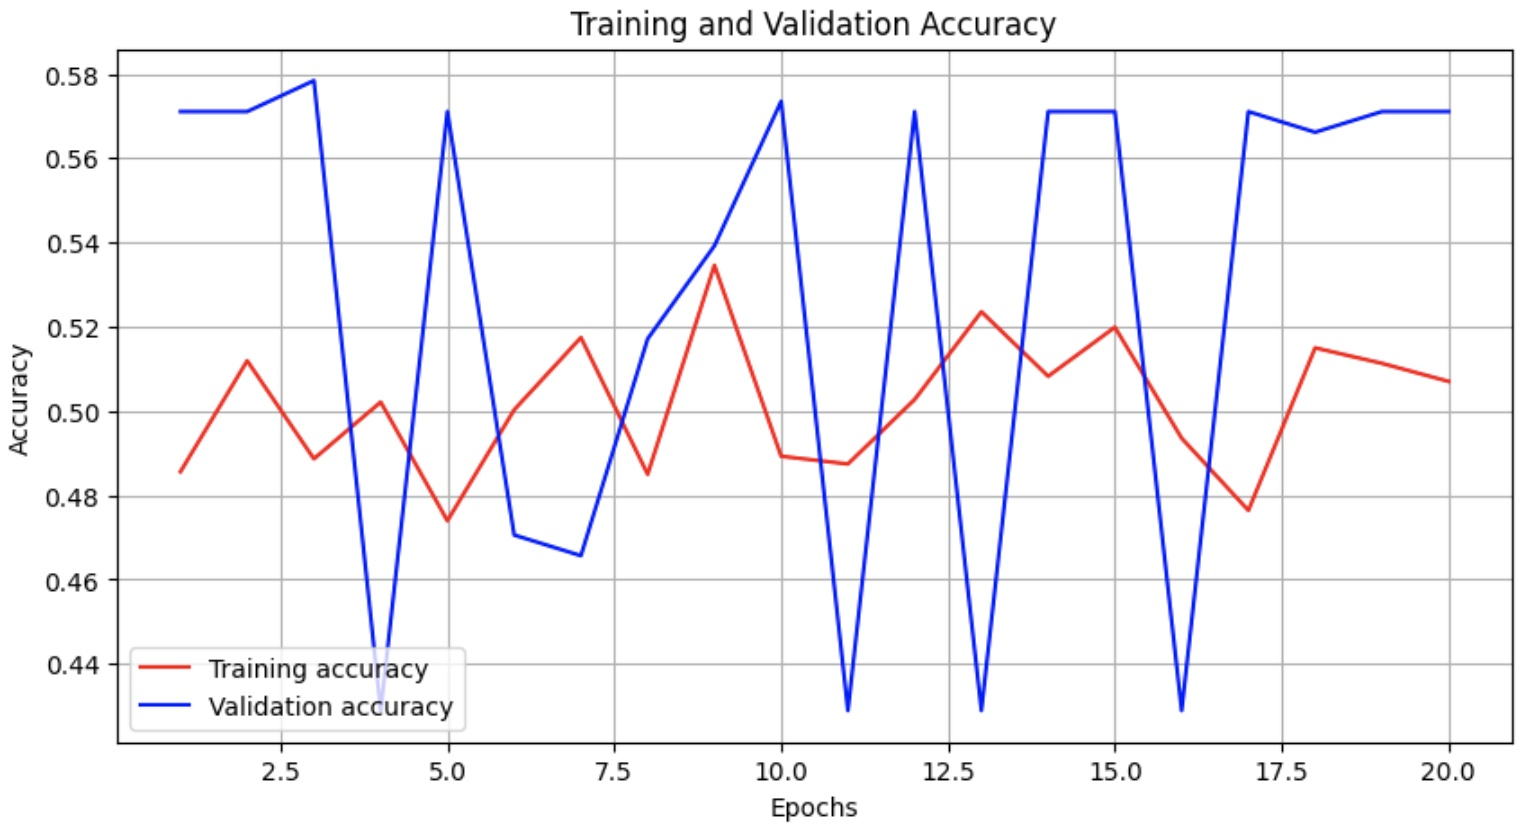
\includegraphics[width=\linewidth]{gramnet51_d1_acc.jpg}
   % \caption{Real faces from dataset 1}
   \label{fig:image2}
\end{minipage}
\caption{Training and validating for GramNet51 on dataset 1}
\label{fig:dataset}
\end{figure*}

\begin{figure*}[t]
\centering
\begin{minipage}{0.45\linewidth}
   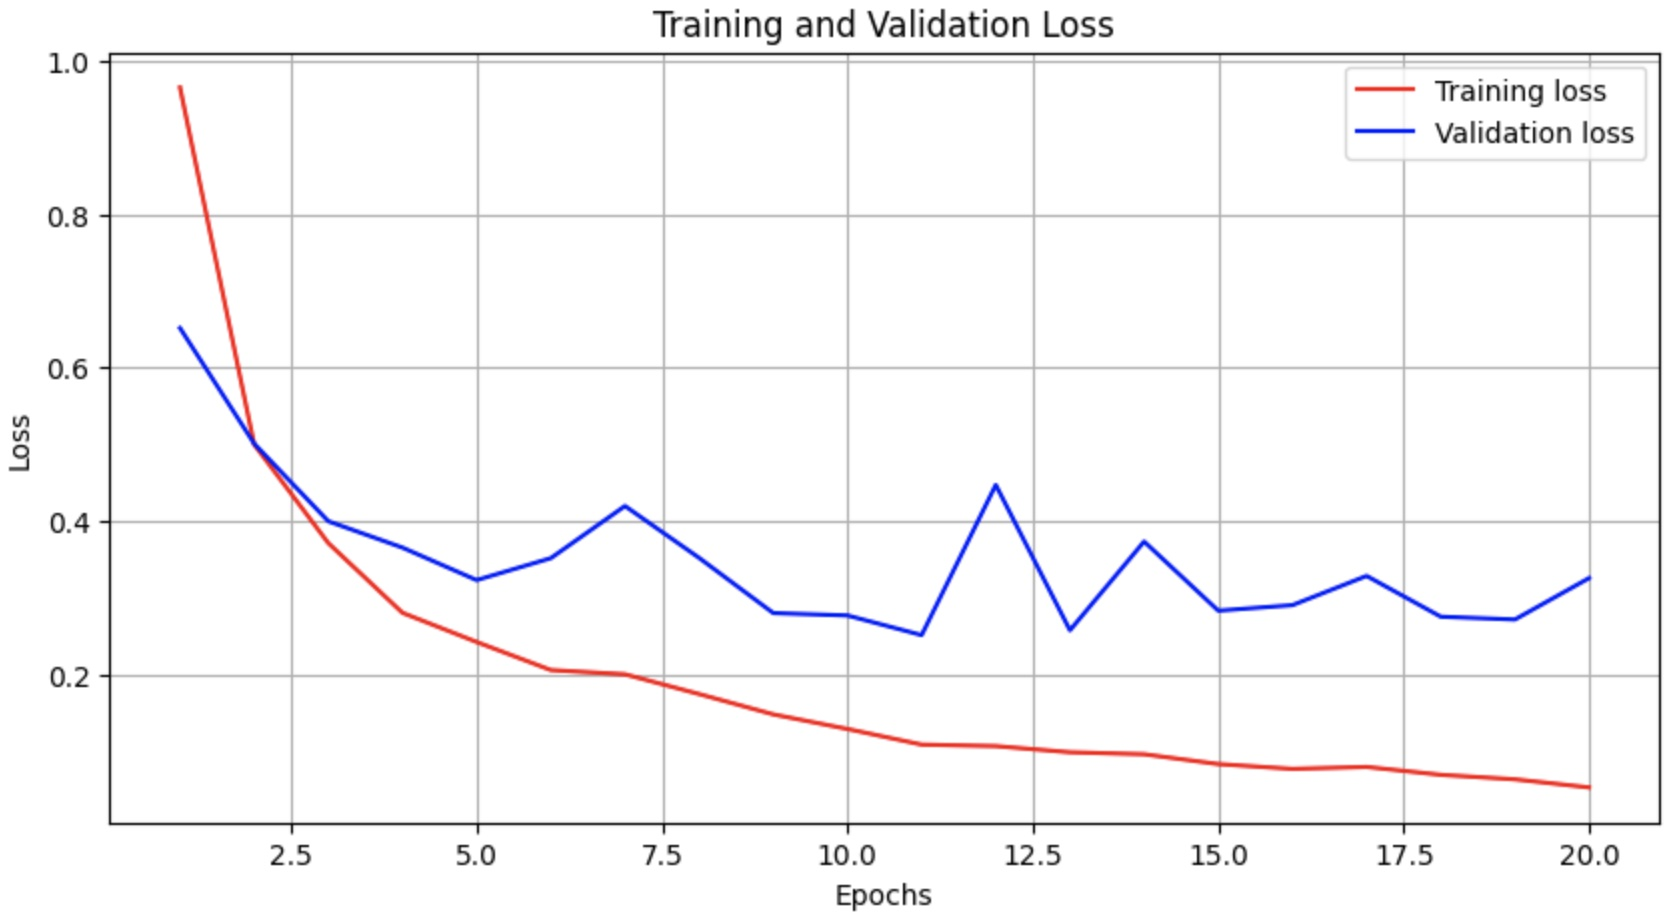
\includegraphics[width=\linewidth]{gramnet51_d2_loss.jpg}
   % \caption{Fake faces from dataset 1}
   \label{fig:image1}
\end{minipage}
\hfill
\begin{minipage}{0.45\linewidth}
   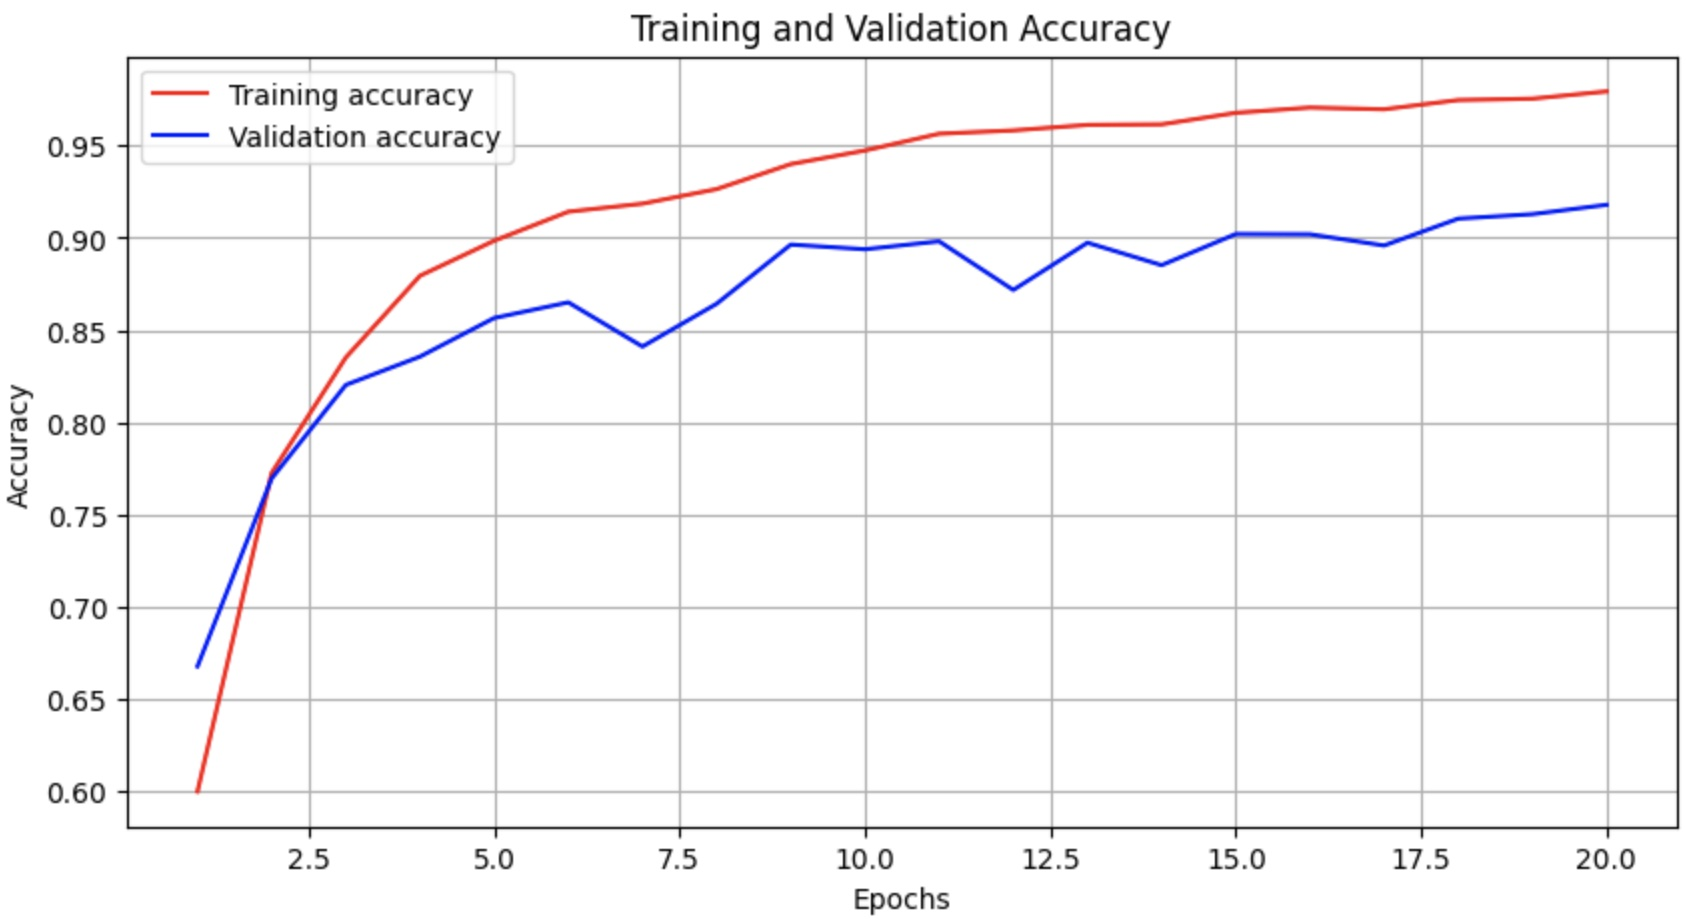
\includegraphics[width=\linewidth]{gramnet51_d2_acc.jpg}
   % \caption{Real faces from dataset 1}
   \label{fig:image2}
\end{minipage}
\caption{Training and validating for GramNet51 on dataset 2}
\label{fig:dataset}
\end{figure*}

\begin{figure*}[t]
\centering
\begin{minipage}{0.45\linewidth}
   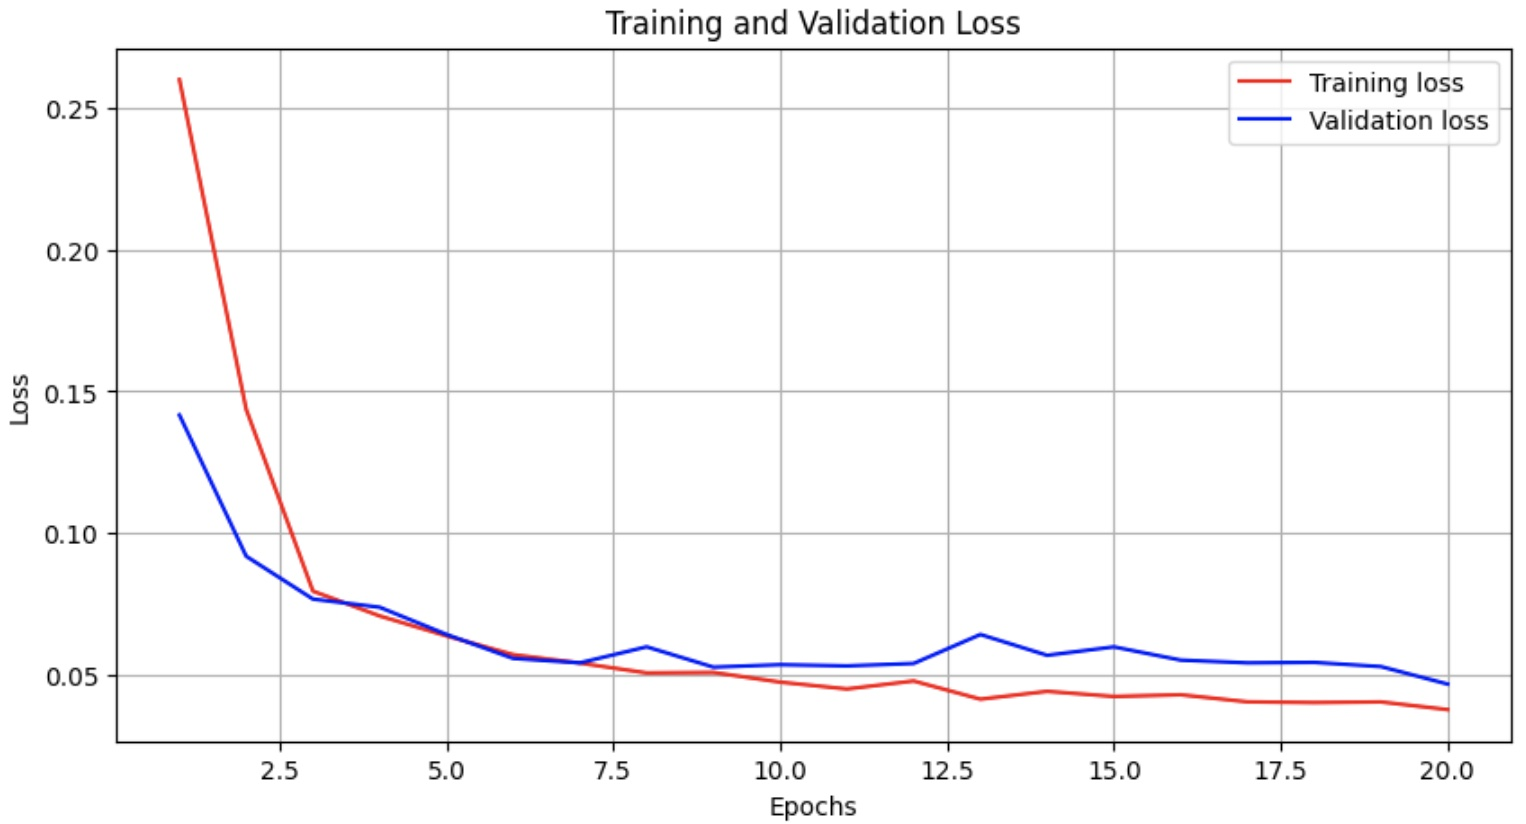
\includegraphics[width=\linewidth]{gramnet51_cd_loss.jpg}
   % \caption{Fake faces from dataset 1}
   \label{fig:image1}
\end{minipage}
\hfill
\begin{minipage}{0.45\linewidth}
   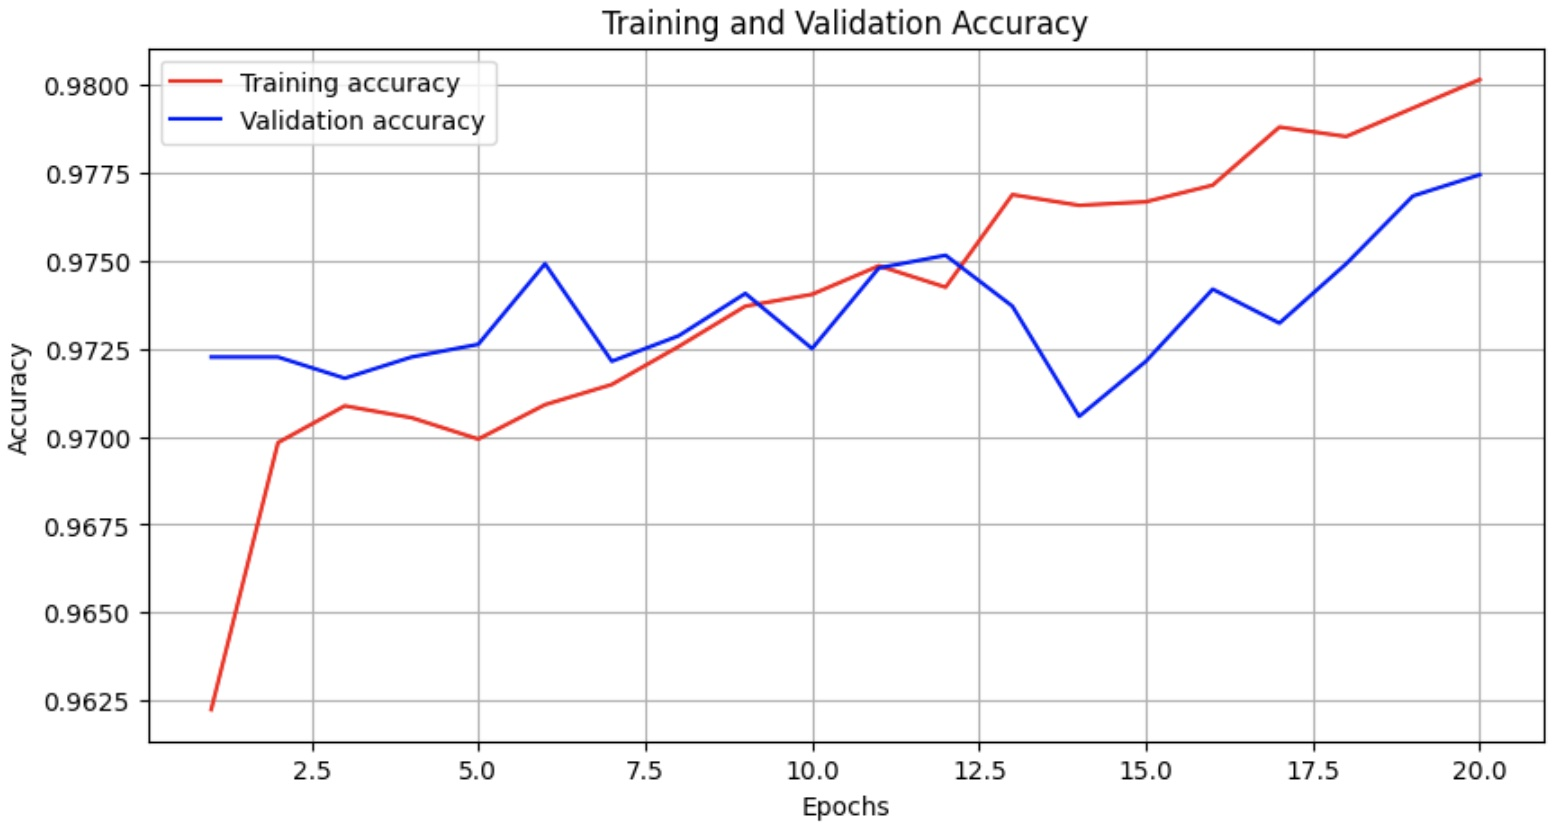
\includegraphics[width=\linewidth]{gramnet51_cd_acc.jpg}
   % \caption{Real faces from dataset 1}
   \label{fig:image2}
\end{minipage}
\caption{Training and validating for GramNet51 on cross-datasets}
\label{fig:dataset}
\end{figure*}

% \begin{figure*}[t]
% \centering
% \begin{minipage}{0.45\linewidth}
%    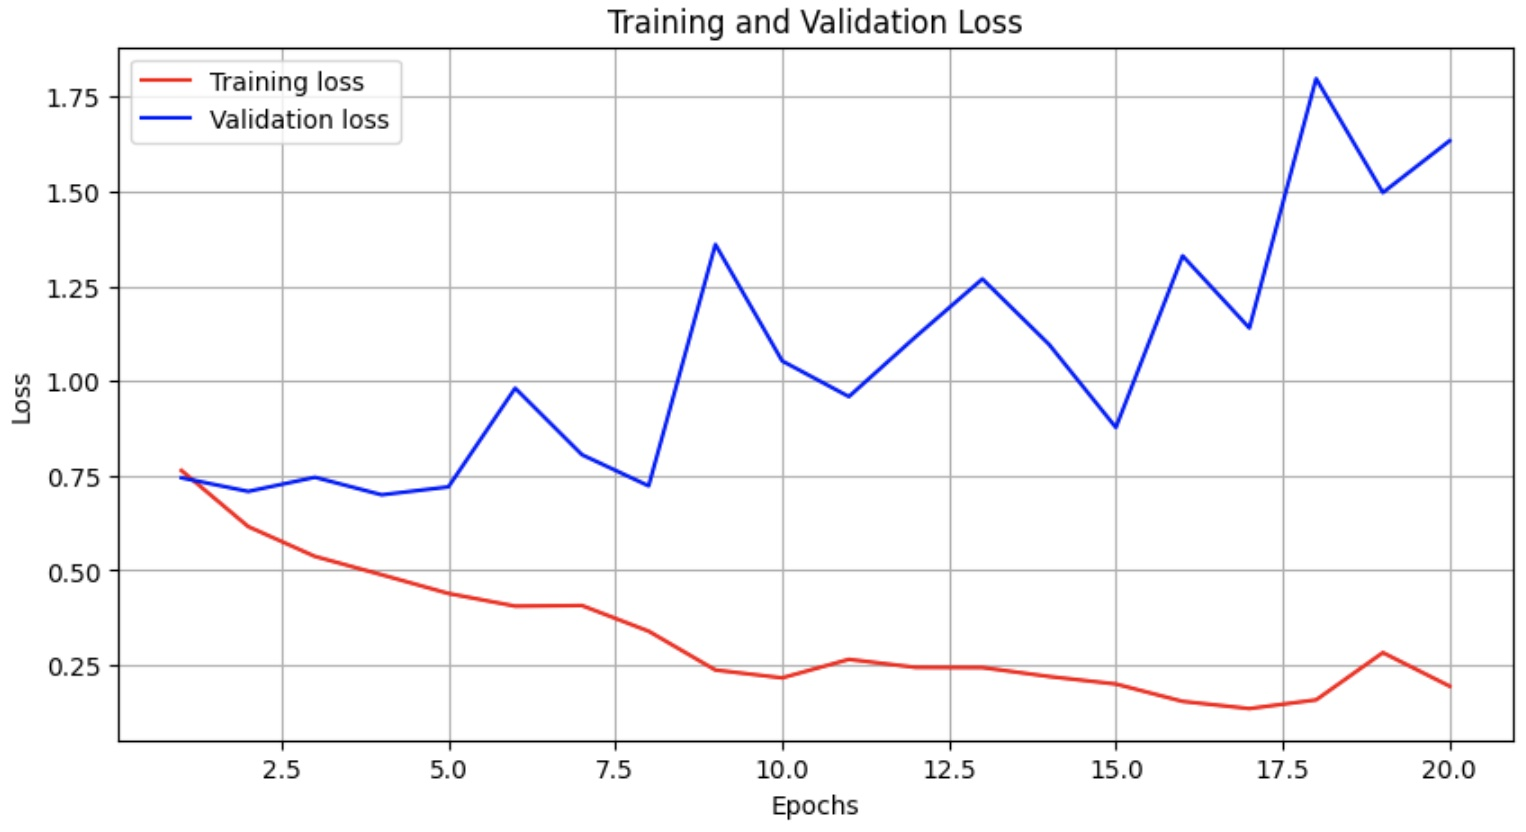
\includegraphics[width=\linewidth]{mobilenetv2_d1_loss.jpg}
%    % \caption{Fake faces from dataset 1}
%    \label{fig:image1}
% \end{minipage}
% \hfill
% \begin{minipage}{0.45\linewidth}
%    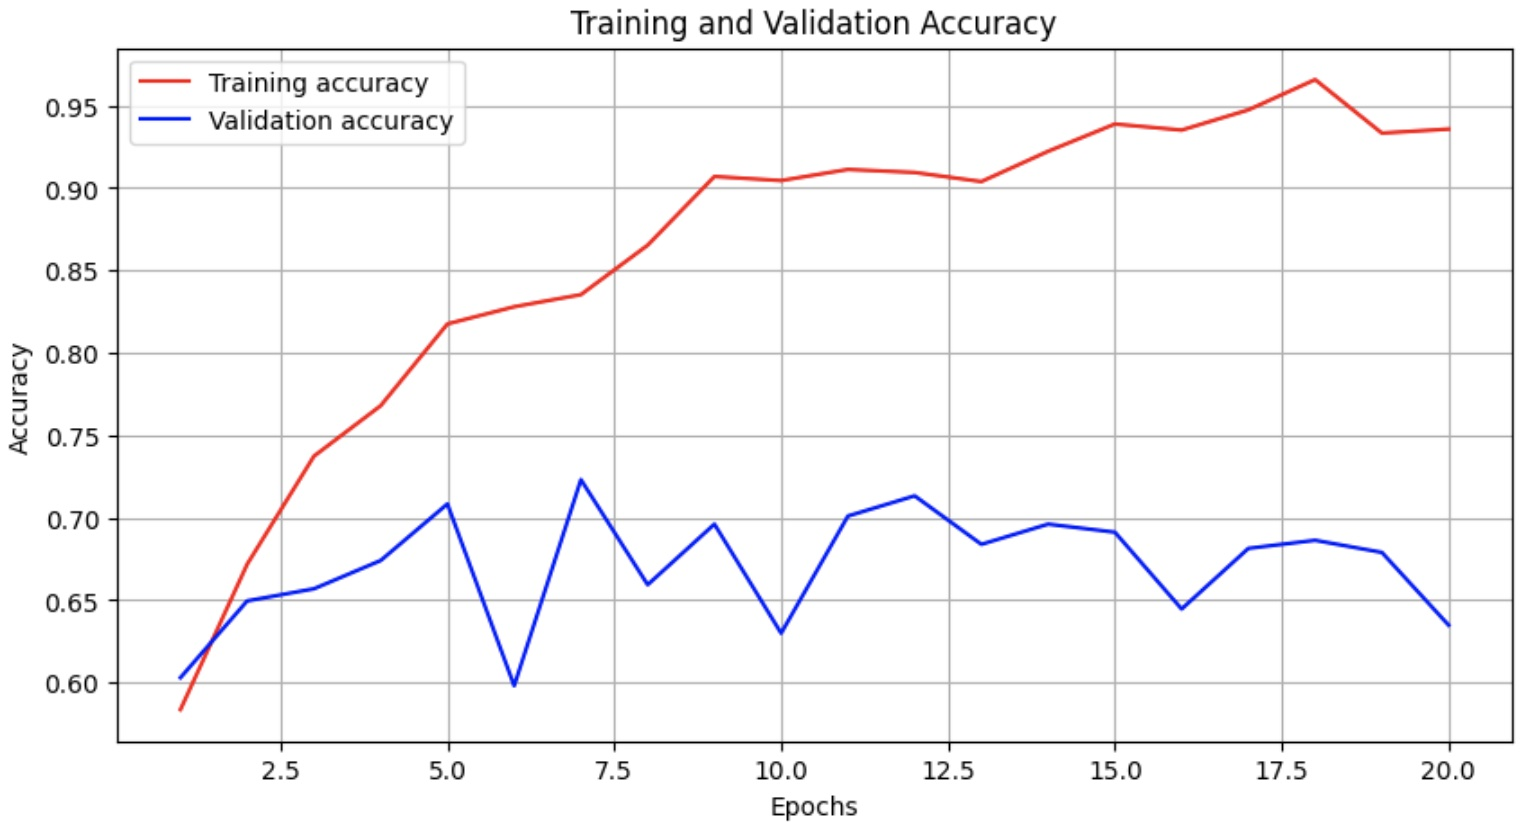
\includegraphics[width=\linewidth]{mobilenetv2_d1_acc.jpg}
%    % \caption{Real faces from dataset 1}
%    \label{fig:image2}
% \end{minipage}
% \caption{Training and validating for MobileNetV2 on dataset 1}
% \label{fig:dataset}
% \end{figure*}

% \begin{figure*}[t]
% \centering
% \begin{minipage}{0.45\linewidth}
%    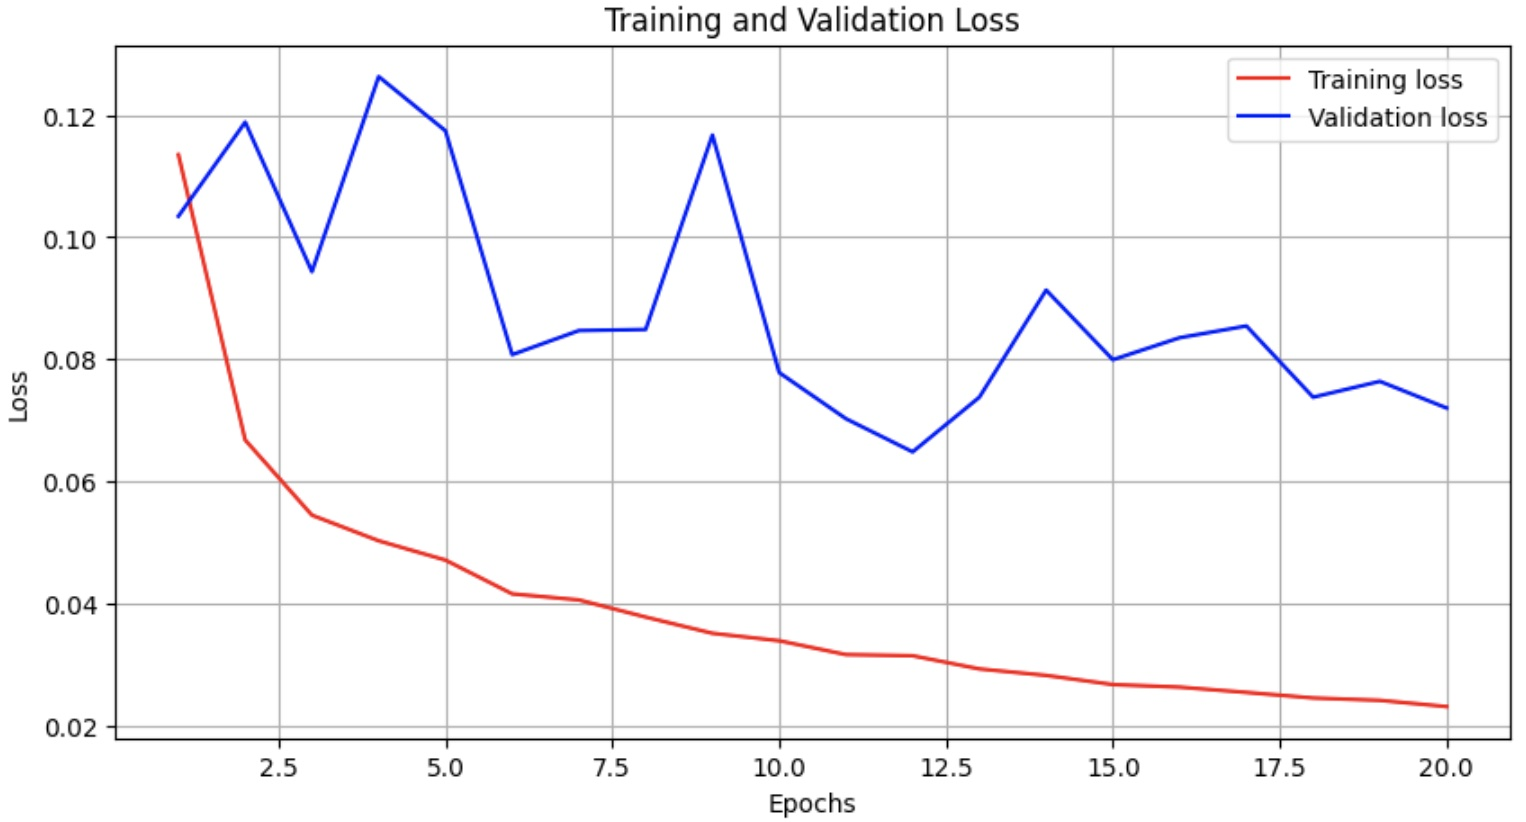
\includegraphics[width=\linewidth]{mobilenetv2_d2_loss.jpg}
%    % \caption{Fake faces from dataset 1}
%    \label{fig:image1}
% \end{minipage}
% \hfill
% \begin{minipage}{0.45\linewidth}
%    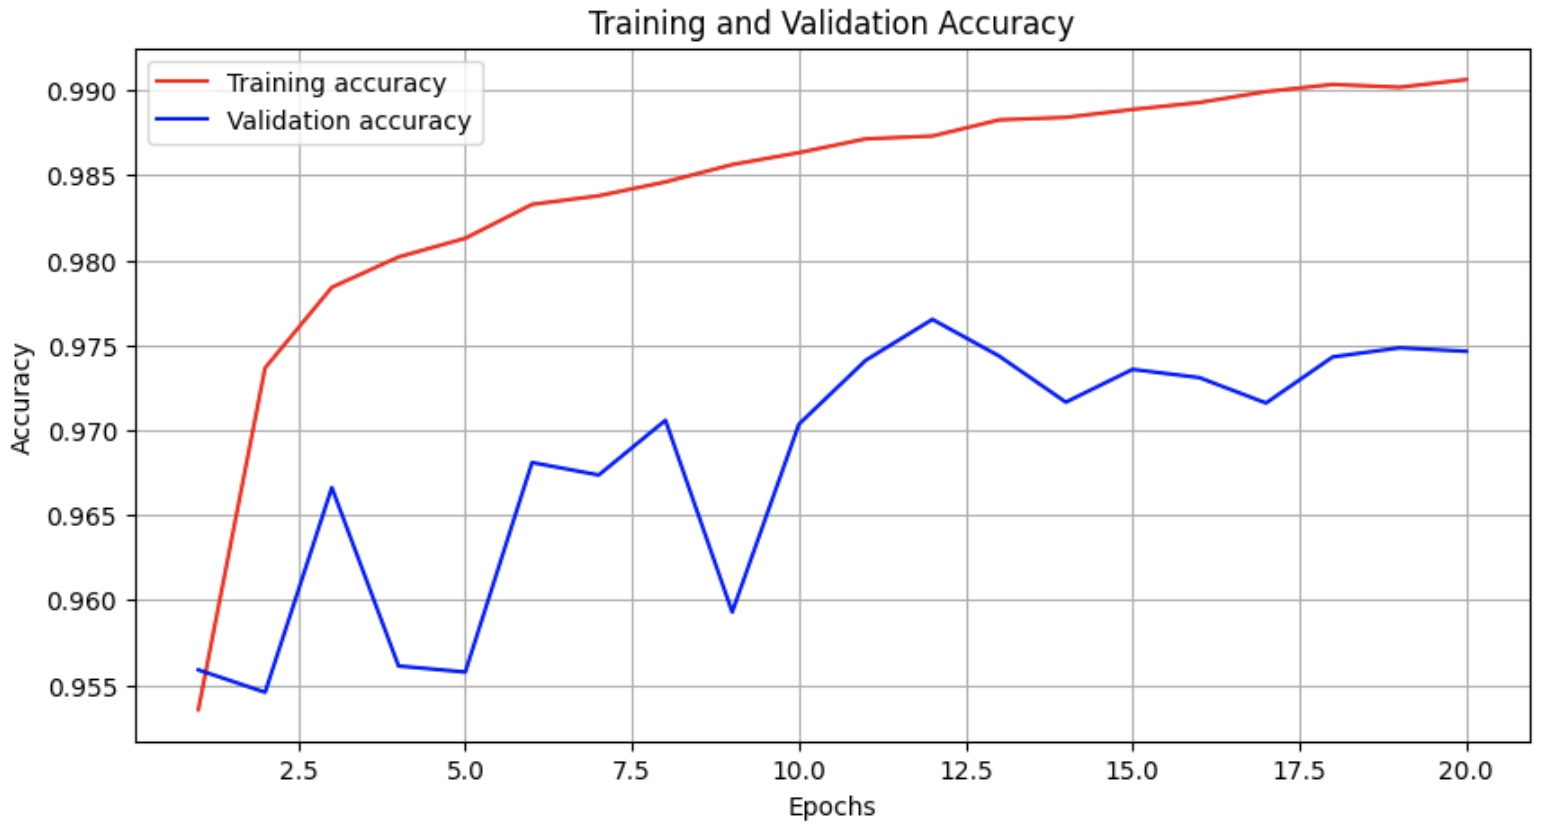
\includegraphics[width=\linewidth]{mobilenetv2_d2_acc.jpg}
%    % \caption{Real faces from dataset 1}
%    \label{fig:image2}
% \end{minipage}
% \caption{Training and validating for MobileNetV2 on dataset 2}
% \label{fig:dataset}
% \end{figure*}

\begin{figure*}[t]
\centering
\begin{minipage}{0.45\linewidth}
   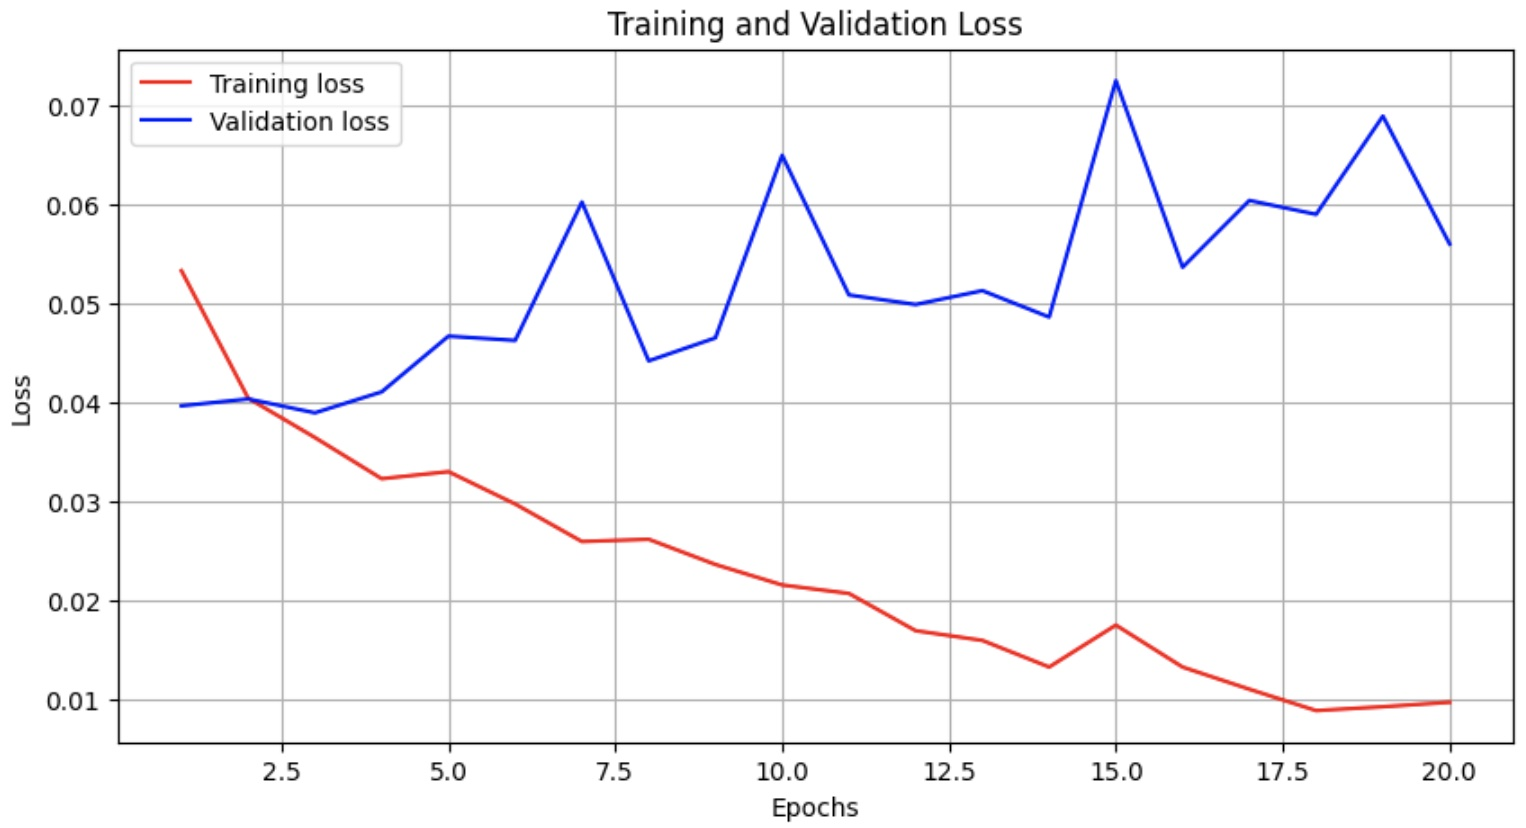
\includegraphics[width=\linewidth]{mobilenetv2_cd_loss.jpg}
   % \caption{Fake faces from dataset 1}
   \label{fig:image1}
\end{minipage}
\hfill
\begin{minipage}{0.45\linewidth}
   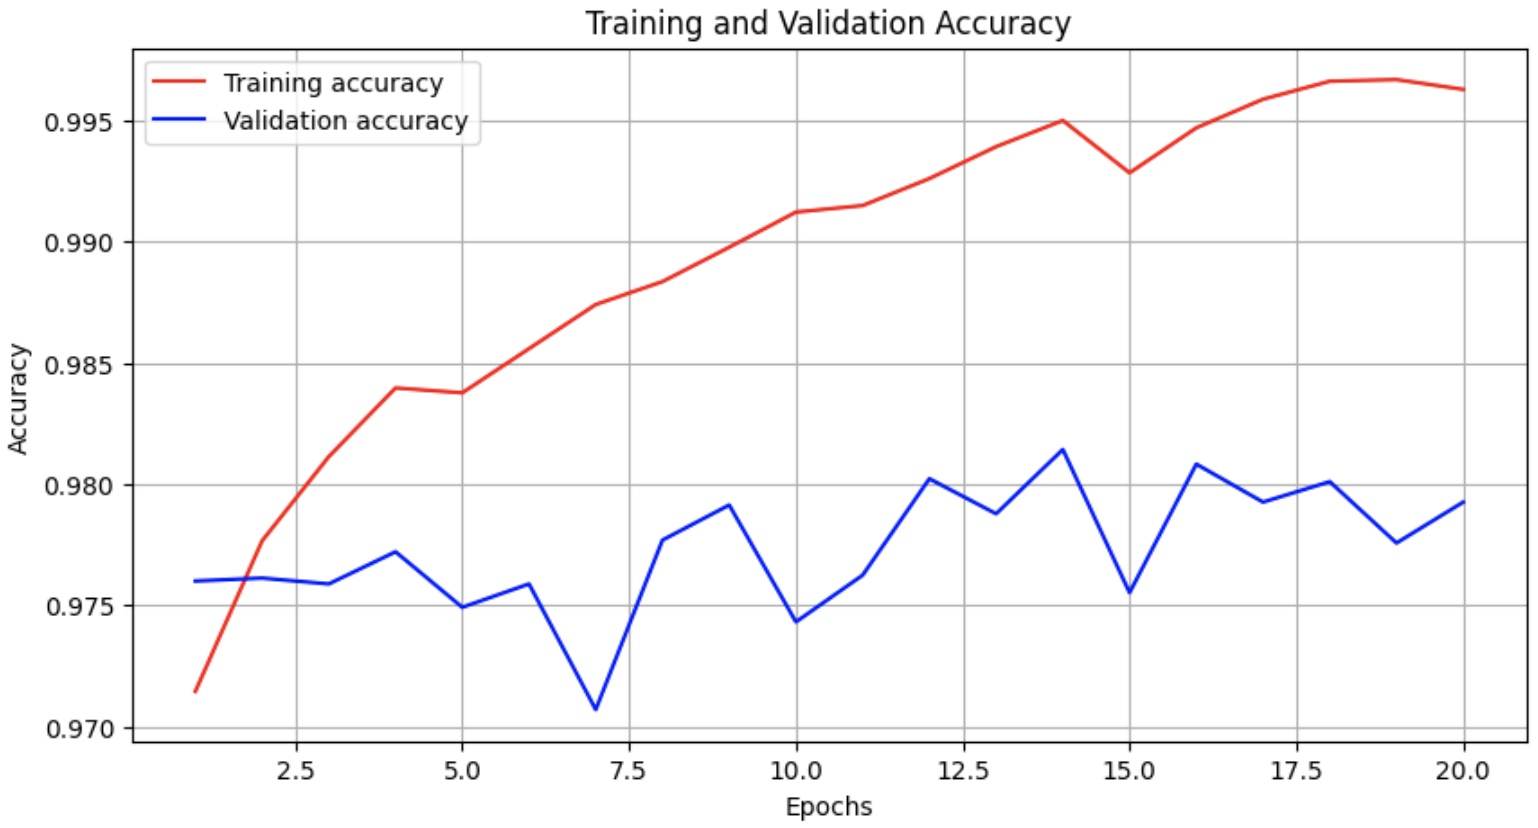
\includegraphics[width=\linewidth]{mobilenetv2_cd_acc.jpg}
   % \caption{Real faces from dataset 1}
   \label{fig:image2}
\end{minipage}
\caption{Training and validating for MobileNetV2 on cross-datasets}
\label{fig:dataset}
\end{figure*}

\section{Findings}
\textbf{Impact of Dataset Quality on Model Performance:} The quality and characteristics of the dataset significantly influence the efficacy of predictive models. This is exemplified in our research, where Dataset 2 outperforms Dataset 1 due to its larger size and greater complexity. Such attributes contribute to enhanced learning opportunities and model performance.\\

\textbf{ Enhancing Model Generalization through Cross-Dataset Training:} We employed cross-dataset training and validation techniques to bolster the generalization capabilities of our model. This method proved to be exceptionally effective in enhancing model performance across varied data sources, demonstrating its utility in creating robust machine learning models.\\

\textbf{ Efficacy of Gram Block Design:} The incorporation of Gram Blocks for capturing more global facial features was validated in our experimental results. This architectural innovation contributed to a noticeable improvement in accuracy, underscoring the value of integrating global feature recognition capabilities in neural network designs.

\section{Conclusion}
In conclusion, we implemented and evaluated GramNet alongside conventional CNN models, including a comparison with the pre-trained MobileNetV2, across two distinct datasets and through cross-dataset experiments. Our findings reveal that employing cross-dataset training significantly enhances the generalization capabilities of our models, demonstrating their robustness across diverse data sources. Furthermore, the GramBlock architecture, designed to capture global facial features, has proven to be highly effective, substantially elevating the accuracy of our models.

Looking forward, we are excited about the prospects of leveraging Generative AI models, such as StyleGAN, to develop more robust datasets. Specifically, we aim to generate advanced synthetic datasets based on high-resolution sources like CelebA-HQ and FFHQ. This approach will not only enrich our training data but also provide deeper insights into the dynamics of facial feature recognition and the overall scalability of our current models in more complex and varied scenarios.


{\bf Make sure to update the paper title and paper ID in the appropriate place in the tex file.}

All text must be in a two-column format. The total allowable width of the text
area is $6\frac78$ inches (17.5 cm) wide by $8\frac78$ inches (22.54 cm) high.
Columns are to be $3\frac14$ inches (8.25 cm) wide, with a $\frac{5}{16}$ inch
(0.8 cm) space between them. The top margin should begin
1.0 inch (2.54 cm) from the top edge of the page.  The bottom margin should be
1-1/8 inches (2.86 cm) from the bottom edge of the page for $8.5 \times
11$-inch paper; for A4 paper, approximately 1-5/8 inches (4.13 cm) from the
bottom edge of the page.

Please number all of your sections and any displayed equations.  It is important
for readers to be able to refer to any particular equation.

Wherever Times is specified, Times Roman may also be used.  Main text should be
in 10-point Times, single-spaced. Section headings should be in 10 or 12 point
Times.  All paragraphs should be indented 1 pica (approx. 1/6 inch or 0.422
cm).  Figure and table captions should be 9-point Roman type as in
Figure~\ref{fig:onecol}.


List and number all bibliographical references in 9-point Times, single-spaced,
at the end of your response. When referenced in the text, enclose the citation
number in square brackets, for example~\cite{Authors14}.  Where appropriate,
include the name(s) of editors of referenced books.

\begin{figure}[t]
\begin{center}
\fbox{\rule{0pt}{1in} \rule{0.9\linewidth}{0pt}}
   %\includegraphics[width=0.8\linewidth]{egfigure.eps}
\end{center}
   \caption{Example of caption.  It is set in Roman so that mathematics
   (always set in Roman: $B \sin A = A \sin B$) may be included without an
   ugly clash.}
\label{fig:long}
\label{fig:onecol}
\end{figure}


%-------------------------------------------------------------------------
\subsection{Illustrations, graphs, and photographs}

All graphics should be centered.  Please ensure that any point you wish to make is resolvable in a printed copy of the response.  Resize fonts in figures to match the font in the body text, and choose line widths which render effectively in print.  Many readers (and reviewers), even of an electronic copy, will choose to print your response in order to read it.  You cannot insist that they do otherwise, and therefore must not assume that they can zoom in to see tiny details on a graphic.

When placing figures in \LaTeX, it's almost always best to use \verb+\includegraphics+, and to specify the  figure width as a multiple of the line width as in the example below



{\small\begin{verbatim}
   \usepackage[dvips]{graphicx} ...
   \includegraphics[width=0.8\linewidth]
                   {myfile.eps}
\end{verbatim}
}

\section{Conclution}

{\small
\bibliographystyle{ieee_fullname}
\bibliography{egbib}
}

\end{document}
